\documentclass[UTF8]{ctexart}
\usepackage{xeCJK}
%\setmainfont{Noto Sans CJK SC}
\setCJKmainfont[BoldFont=Noto Sans S Chinese Bold Bold]{Noto Sans S Chinese Regular}
\usepackage{geometry}
\usepackage{booktabs}
\geometry{a4paper, left=2cm, right=2cm,top=2cm,bottom=2cm}
\usepackage{amsmath}
\usepackage{pifont}
\usepackage{hyperref}
\usepackage{mathrsfs}
\usepackage{graphicx}
\usepackage{wrapfig}
\newcommand{\minisection}{\subsection}
\newcommand{\backdoc}{\normalsize}

\title{Part2	Polarization}
\author{Xiao Liang}
\date{\today}

\begin{document}
	\maketitle
	\tableofcontents
	\numberwithin{equation}{section}
	%\CJKfontspec{Noto Sans Mono CJK SC}
	\CJKfontspec[BoldFont=Noto Sans S Chinese Bold Bold]{Noto Sans S Chinese Regular}
	\section{偏振形式}
	\subsection{随机偏振}
	
	\normalsize
	随机偏振是各向同性的表现,是众多不相关光子叠加后的产物,有时也被称为无偏光和自然光。
	
	\subsection{椭圆偏振}
	
	\backdoc
	椭圆偏振可分为一般椭圆偏振、线偏振和圆偏振。线偏振和圆偏振都是特殊的椭圆偏振。不同的偏振形式根源是两个正交轴上的电场分量(磁场同理)存在相位差导致,具体如下:
	\begin{equation}
	\begin{array}{l}{\vec{E}(z, t)=\vec{E}_{x}(z, t)+\vec{E}_{y}(z, t)} \\ {=\hat{i} E_{0 x} \cos (k z-\omega t)+\hat{j} E_{0 y} \cos (k z-\omega t+\varepsilon)}\end{array}\label{equ_1.1}
	\end{equation}
	
	(1)当$\varepsilon=$0 or $\pi$时,呈现的即是线性偏振光,此时光波幅值会发生周期性变化。
	
	(2)当$E_{0 \mathrm{x}}=E_{0 \mathrm{y}}$且$\varepsilon=\pm\pi/2$时,呈现的即是圆偏振光,此时光波幅值不会发生变化,但方向会发生周期性变化,具体是:当$\varepsilon=\pi/2$时,为左旋圆偏振;当$\varepsilon=-\pi/2$时,为右旋圆偏振。
	
	(3) 一般椭圆偏振情况可由式\ref{equ_1.1}推出,椭圆方程为:
	\begin{equation}
	\left(\frac{E_{y}}{E_{0 y}}\right)^{2}+\left(\frac{E_{x}}{E_{0 x}}\right)^{2}-2\left(\frac{E_{x}}{E_{0 x}}\right)\left(\frac{E_{y}}{E_{0 y}}\right) \cos \varepsilon=\sin ^{2} \varepsilon
	\end{equation}
	
	考虑此椭圆方程是标准椭圆方程$\left(\frac{E_{y}^{\prime}}{E_{0 y}^{\prime}}\right)^{2}+\left(\frac{E_{x}^{\prime}}{E_{0 x}^{\prime}}\right)^{2}=1$经过逆时针旋转$\theta=\alpha$得到的,通过坐标变换和待定系数法可以得到$\alpha$同$\varepsilon$、$E_{0x}^{\prime}$和$E_{0y}^{\prime}$之间的关系如下:
	\begin{equation}
	\tan(2\alpha)=\frac{2E_{0x}^{\prime}E_{0y}^{\prime}\cos\varepsilon}{E_{0x}^{\prime 2}-E_{0y}^{\prime 2}}
	\end{equation}
	
	几种偏振可表达成如下形式:
	
	$\mathscr{P}$-state: Plane- or linear-polarized.
	
	$\mathscr{R}$-state: Right-circular-polarized.

	$\mathscr{L}$-state: Letf-circular-polarized.
	
	$\mathscr{E}$-state: Elliptical-polarized.
	
	它们之间的关系如下:
	\begin{equation}
	\mathscr{P}=\mathscr{R}+\mathscr{L}
	\end{equation}
	\begin{equation}
	\mathscr{E}=a\mathscr{R}+b\mathscr{L}
	\end{equation}
	
	\section{起偏器}
	起偏器是指输入是自然光而输出的偏振光的光学仪器。各式各样的起偏器都基于以下四种基本物理机制:二向色性(选择性吸收)、反射、散射以及双折射。它们都具备一个共同的根本性质,这就是起偏过程必须有某种形式的不对称性。
	
	\subsection{玻璃分光镜}
	
	\backdoc
	利用多片玻璃叠合成的片堆,并使得入射光和玻璃的偏角等于布鲁斯特角,可以得到线偏振光。其中,反射光具有较大的强度,而折射光也具有较好地偏振性。
	
	\subsection{利用二向色性制成的偏振片}
	
	\backdoc
	\textbf{二向色性(Dichroism)}是指某些各向异性的晶体对不同振动方向的偏振光有不同的吸收系数的性质,这是由于晶体中粒子的排列导致的。参考偶极子在电磁场中振荡的模型可以得知,如果晶体粒子的振动方向较多地位于某一特定方向,那这个方向上的激发电场就会较弱,因而表现在这个方向上具有很强的吸收性。
	
	一般地,晶体的二向色性还与光波波长有关,因此当振动方向互相垂直的两束线偏振白光通过晶体后会呈现出不同的颜色。这就是二向色性这个名称的由来。有些本来各向同性的介质在收到外界作用是会产生各向异性,他们对光的吸收本领也随着光矢量的方向而变,这种性质也叫做二向色性。
	
	目前广泛使用的获得偏振光的器件,是人造的偏振片——H偏振片和K偏振片,都是具有一条可拉伸的导电分子,使得平行于该方向的光被大幅吸收,而垂直于该方向的光可以透过。能够透光的方向被称为它的\textbf{透光轴}。
	
	\subsection{马吕斯定律}
	
	\backdoc
	利用两片相同的偏振片可以检测是否产生了线偏振光。令一束自然光按顺序通过这两片偏振片,前者用以产生线偏振光(被称为\textbf{起偏器}),而后者用以检测偏振光(被称为\textbf{检偏器})。当它们相对转动时,透过两片偏振片的光强就随着两偏振片的透光轴的夹角$\theta$而变化。如果偏振片是理想的,在两片偏振片的光轴方向垂直的情况下,透射光强应该为零。当夹角$\theta$为其他值时,投射光强由下式决定:
	\begin{equation}
	I(\theta)=\frac{c \varepsilon_{0}}{2} E_{0}^{2} \cos ^{2} \theta=I(0) \cos ^{2} \theta
	\end{equation}
	
	此式子得到依赖于光强同电场强度的关系,具体如下:
	\begin{equation}
		\begin{aligned}
	<S>&=\frac{1}{T} \int_{0}^{T} S d t=v \epsilon E^{2} \frac{1}{T} \int_{0}^{T} \cos ^{2}(k r-w t) d t\\
	&=\frac{1}{2} v \epsilon E^{2}=\frac{1}{2} \sqrt{\frac{\epsilon}{\mu}}  E^{2}
		\end{aligned}
	\end{equation}
	
	式(4.6)所表示的关系被称为\textbf{马吕斯定律(Malus's Law)}。由于实际的偏振期间往往不是很理想,自然光投过后得到的是部分偏振光,因此即便两个偏振器件的透光轴互相垂直,透射光强也不为零。这时定义最小透射光强与两偏振器件互相平行时的最大透射光强之比为\textbf{消光比},即:
	\begin{equation}
	f=\frac{I(\pi/2)}{I(0)}
	\end{equation}
	
	\section{晶体的双折射}
	一束单色光(近似考虑)在各向同性介质的界面折射时,折射光只有一束,而且遵守折射定律;然而在各向异性晶体的界面折射时,则一般可产生两束折射光,这种现象被称为\textbf{双折射}。
	
	双折射本质上是晶体对同样的光具有双折射率,从电偶极子的模型来考虑就是电子的振动在不同方向具有不同的本征频率。由于折射波的速度是由E场频率和电子的自然频率或本征频率决定,束缚力的各向异性也就表示为折射率的各向异性。
	
	上文的二向色性是其中特殊的一种。
	
	\subsection{o光和e光}
	
	\backdoc
	两束折射光中,有一束光总是遵守折射定律,即不论入射光束的方位如何,都总是在入射面内,且折射角的正弦和入射角的正弦之比为常数,这束光即是\textbf{o(ordinary)}光。另一束光一般情况下不遵守折射定律,被称为\textbf{e(extraordinary)}光。
	
	\subsection{晶体光轴}
	
	\backdoc
	晶体内存在一个特殊的方向,当光在晶体中沿着这个方向传播时不发生双折射,这个方向就被称为\textbf{晶体光轴}。光轴并不是经过晶体的某一条特定的直线,而是一个方向。在晶体内的每一点,都可以作出一条光轴来。
	
	有些晶体只有一个光轴方向,被称为\textbf{单轴晶体},而自然界大多数晶体都有两个光轴方向,称为\textbf{双轴晶体}。
	
	\subsection{主平面和主截面}
	
	\backdoc
	在单晶体内,由o光和光轴组成的面称为o主平面;由e光和光轴组成的面称为e主平面。一般情况下,o主平面和e主平面不平行。但若光线在由光轴和晶体表面法线组成的平面内入射,则o光和e光都在这个平面内,这个平面也就是它们共同的主平面。这个由光轴和晶体表面法组成的面称为晶体的\textbf{主截面}。
	
	如果用检偏器来检验晶体双折射产生的o光和e光的偏振状态,就会发现它们都是线偏光。o光的电矢量与o主平面垂直,因而总是与光轴垂直;e光的电矢量在e平面内,因而它与光轴的夹角就随着传播方向的不同而改变。由于o主平面和e主平面在一般情况夏并不重合,所以o光和e光的电矢量一般也不互相垂直;只有当主截面是o光和e光的\textbf{共同主截面}时,o光和e光才互相垂直。
	
	\section{双折射的电磁理论(唯象)}
	\subsection{o光和e光的传播}
	
	\backdoc
	因为\textbf{E}场是垂直于光轴的,我们假定波前(它在初始位置相当于表面)上的每一点都起到球面子波的作用,并且都同相。可以推测,只要\textbf{子波的电场在每一个点上都垂直于光轴},那么在晶体内部的任何方向,子波都以一个速度向外扩展,就好像在各向同性媒介中一样。
	
	考虑一个场,\textbf{E}平行于主截面,有一个分量垂直于光轴,还有一个分量平行于光轴。由于媒介是双折射媒介,偏振方向平行于光轴的某一频率的光以速率$v_{p}$传播,而$v_{p} \neq v_{v}$,在这种情况下,某一个方向上的波传播速度更快,使得合成的次级子波偏离球面变为椭球面。全部椭球面子波的包络是一个平行于入射波的平面波的一部分,然而,在通过晶体的时候,这个平面波显然将发生一个侧向移动。光束方向仍然平行于连接每个子波的原点与子波和平面包络切点的连线,这个方向称为\textbf{射线方向},它相当于\textbf{能量传播的方向}。
	
	从电磁理论的角度来考虑。在电介质内,存在电偶极矩,电介质内部的场,由于包含了感生电场而发生了变化,因此要引入一个新的量——点位移矢量\textbf{D}。在各向同性媒介中\textbf{D}和\textbf{E}通过一个标量联系起来,两者总是平行的,但在各向异性晶体中,两者通过一个张量联系,不会总是平行的。通过将麦克斯韦方程用于传播问题,会发现波阵面内振动的场是\textbf{D}和\textbf{B},而不是原来的\textbf{E}和\textbf{B}。垂直于等相面的传播矢量\textbf{k}现在垂直于\textbf{D}而不是\textbf{E}。然而,射线方向对应于坡印廷矢量 $\mathbf{S}=c^{2} \epsilon_{\mathbf{0}} \mathbf{E} \times \mathbf{B}$ 的方向,后者通常和\textbf{k}的方向不一样。只有当\textbf{E}和\textbf{D}都平行于或者都垂直于光轴时,它们才会共线。
	
	这意味着o光子波将遇到等效的各向同性媒介,所以是球形的,\textbf{S}和\textbf{k}共线。相反,对于e光子波,只有在平行或垂直于光轴的方向上,\textbf{S}和\textbf{k}才会平行。在子波的所有其他点,和椭球相切的是\textbf{D},因此永远是\textbf{D}落在包络上或在晶体内的合成的平面波阵面上。
	
	\section{散射和偏振}
	\subsection{散射}
	
	\backdoc
	当电磁波投射到原子或者分子上时,它和束缚电子云相互作用,把能量交给原子。只有当振动频率等于原子的共振频率附近时,振荡幅度才很大。处于共振时原子的行为可以做如下简单描述:起初在基态,吸收了一个光子之后,跃迁到激发态。在光密媒介中,原子倾向于把这个多余的能量以热的形式放出,从而回到基态。在稀薄气体中原子一般放出\textbf{一个}光子而向下跃迁,这个效应叫做\textbf{共振辐射}。
	
	而处于非共振频率上时,原子(偶极子)从入射波中取走能量,随后又把这能量的一部分再发射出来,这个过程就叫做\textbf{散射}。它是在反射、折射和衍射中起作用的基本物理机制。
	
	\subsection{散射引起的偏振}
	
	\backdoc
	可以将自然光看做正交的不相干线偏振光的叠加,此时散射光等价于两个方向上线偏振光结果的叠加。在前进方向上散射光是完全不偏振的;偏离前进方向为部分偏振,偏离的角度增加偏振的程度也加大。当观察方向垂直于主光束时,散射光是完全偏振的。
	
	\section{推迟器}
	推迟器原理上十分简单。通过令两个相干的$ \mathscr{R} $态中,设法使一个$ \mathscr{R} $态比另一个$ \mathscr{R} $态落后一个给定的相位,从而改变光束的偏振形态。
	
	\subsection{波片}
	
	\backdoc
	利用晶体的双折射特性便可以制作波片。如果入射的单色平面波的\textbf{E}场具有平行于光轴和垂直于光轴的分量,则在晶体中将有两个波传播。由于$v_{ \|}>v_{\perp}, n_{0}>n_{e}$,所以e波将比o波更快地通过晶片。在通过厚度为d的晶片后,总的电磁波是e波和o波的叠加,而它们之间存在相对相位差。留意,它们都是频率相同的简谐波,\textbf{E}场互相正交,现在,相对的光程差为:
	\begin{equation}
\Lambda=d\left(\left|n_{o}-n_{e}\right|\right)
	\end{equation}
	
	\noindent 因为$\Delta \varphi=k_{0} \Lambda$,
	\begin{equation}
\Delta \varphi=\frac{2 \pi}{\lambda_{0}} d\left(\left|n_{o}-n_{e}\right|\right)
	\end{equation}
	
	\noindent 式中$\lambda_{0}$是真空中的波长(含有折射率之差的绝对值的形式是最普遍的表述方法)。出射光的偏振态显然依赖于入射波两个正交场的分振幅,当然也依赖于相位差$\Delta \varphi$。
	
	根据使o光和e光的相对位相差不同可将常用波片分为以下几种:
	
	(1)全波片。
	
	由于全波片只是针对某一特定波长而言的,所以这类推迟器是有颜色区别的。只有特定波长的光保持偏振形式,被检偏器吸收,其余的光都会改变偏振形式,一部分被检偏器吸收,最后以消光的互补色投射出来。
	
	在负单轴推迟器中的光轴方向常常被称为\textbf{快轴},而垂直于它的方向则被称为\textbf{慢轴}。在正单轴推迟器中情况则要反过来。由此可见,历史上以光轴为慢轴为\textbf{正}。
	
	(2)半波片
	
	使o光和e光的相对相位差为$\pi$,可以改变椭圆偏振光的方向,还可以把右旋的圆偏振光或椭圆偏振光变为左旋,把左旋的变为右旋。
	
	(3)四分之一波片
	
	使o光和e光的相对相位差为$\frac{\pi}{2}$,可以将线偏振光变成椭圆偏振光,反之亦然。
	
	补充:菲涅尔斜方体通过两次反射使得两个分量的相对位移为$\frac{\pi}{2}$,可以视为\textbf{全色}的四分之一波片。
	
	\subsection{补偿器}
	
	\backdoc
	补偿器是\textbf{能够使光波产生可以控制的推迟的光学器件},不像$\Delta \varphi$固定的波长片,补偿器的相对位移差是可以连续变化的。它由两个独立的斜楔组合而成,两个斜楔的o光和e光恰好相反,因而斜楔的厚度差就可以决定相对位移差,具体如下:
	\begin{equation}
\Delta \varphi=\frac{2 \pi}{\lambda_{0}}\left(d_{1}-d_{2}\right)\left(\left|n_{o}-n_{e}\right|\right)
	\end{equation}
	
	\section{圆起偏器}
	一个恰当取向的线起偏器和一个四分之一波片的串接组合可以起到圆偏振片的作用。这两个元件完全独立地作用,其中一个可以是双折射型的,另一个可能是反射型的。
	
	如果将线起偏器放在两个推迟器中间,一个推迟器取向为$+45^{\circ}$,另一个取向为$-45^{\circ}$,那么,光从一端进去会得到$\mathscr{R}$态,从另一边进去会得到$\mathscr{L}$态。
	
	圆起偏器也可以用作检偏器。\textbf{左旋圆偏振光从输出端射入左旋圆起偏器时将会透射,而右旋圆偏振光将无法从输出端通过左旋起偏器},反之亦然。
	
	\section{旋光性和感生光学效应——光调制器}
	线偏振光传播时可能会出现振动面连续地转动的现象,这种现象被称为“旋光性”。旋转分为右旋和左旋两种,判断标准同圆偏振光。
	
	\subsection{有关旋光性的模型和公式}
	
	\backdoc
	旋光性是非常复杂的一个现象,它虽然可以用经典电磁理论来处理,但实际上需要量子力学的解。
	
	从唯象的角度来考虑,可以分解入射的线偏振光为$\mathscr{R}$态和$\mathscr{L}$态的叠加,同时认为这两种偏振光的传播速度不相同。旋光性的材料具有\textbf{圆双折射},也即有两个折射率。我们可以如此表示:
	\begin{equation}
	\begin{aligned}
	\mathbf{E}_{\mathscr{R}}&=\frac{E_{0}}{2}\left[\hat{\mathbf{i}} \cos \left(k_{\mathscr{R}} z-\omega t\right)+\hat{\mathbf{j}} \sin \left(k_{\mathscr{R}} z-\omega t\right)\right]\\
	\mathbf{E}_{\mathscr{L}}&=\frac{E_{0}}{2}\left[\hat{\mathbf{i}} \cos \left(k_{\mathscr{L}} z-\omega t\right)-\hat{\mathbf{j}} \sin \left(k_{\mathscr{L}} z-\omega t\right)\right]
	\end{aligned} 
	\end{equation}
	
	由于$\omega$是常数,$k_{\mathscr{R}}=k_{0} n_{\mathscr{R}}$,$k_{\mathscr{L}}=k_{0} n_{\mathscr{L}}$,合成的扰动为$\mathbf{E}=\mathbf{E}_{\mathscr{R}}+\mathbf{E}_{\mathscr{L}}$,经过三角运算后,变为
	\begin{equation}
	\begin{aligned}
	\mathbf{E}=&E_{0} \cos \left[\left(k_{\mathscr{R}}+k_{\mathscr{L}}\right) z / 2-\omega t\right]\\
	&\left[\hat{\mathbf{i}} \cos \left(k_{\mathscr{R}}-k_{\mathscr{L}}\right) z / 2+\hat{\mathbf{j}} \sin \left(k_{\mathscr{R}}-k_{\mathscr{Z}}\right) z / 2 \right]
	\end{aligned}
	\end{equation}
	
	由于左旋光和右旋光的折射率不同,导致合成的结果虽然确定是线性偏振光,但同水平方向的夹角始终在发生变化。考虑振动面旋转角度$\beta=-\left(k_{\mathscr{R}}-k_{\mathscr{L}}\right) z / 2$,介质厚度为d,振动面旋转的角度为:
	\begin{equation}
	\beta=-\frac{\pi
	d}{\lambda_{0}}\left(n_{\mathscr{L}}-n_{\mathscr{R}}\right)
	\end{equation}
	
	\noindent 其中$n_{\mathscr{L}}>n_{\mathscr{R}}$时为右旋,$n_{\mathscr{R}}>n_{\mathscr{L}}$为左旋。
	
	考虑一个更加贴合实质的简化的模型。把光学各向异性视作各向异性振子的分布,振子的振动方向和驱动的\textbf{E}场成某一角度。可以设想旋光材料中的电子被迫绕一条螺旋线运动,此时分子的图像就像一条导电的螺旋线。
	
	在这样的情况下,我们可以预计,入射波根据它遇到的分子螺旋情况的不同,和样品的相互作用也就不同,进而导致了波的左旋和右旋分量有不同的折射率。
	
	\subsection{感生光学效应——光调制器}
	现在考虑法拉第效应,又被称为磁光效应,这是因为光在媒介中传播的方式会受到外加磁场的影响。类似旋光性,振动面旋转的角度$\beta$(以弧分来量度)由经验关系式给出:
	\begin{equation}
		\beta=\mathscr{V} B d
	\end{equation}
	
	\noindent 式中$B$为静磁通量(通常用高斯作单位),$d$是所穿越的媒质的长度(单位为cm),$\mathscr{V}$是比例因子,叫做\textbf{费尔德常数}。
	
	我们约定,正的费尔德常数对应这样一种(抗磁)材料:当光的传播方向平行于所加的\textbf{B}场时法拉第效应时左旋的,反平行于\textbf{B}时为右旋的。同自然的旋光性有区别,因为自然的旋光性不会存在这样的倒转。
	
	法拉第效应是磁光效应,现在来考虑电光效应。第一个电光效应是克尔效应:一个各向同性的透明媒介置于电场\textbf{E}中就变成双折射的了,媒介具有单轴晶体的特征,其光轴对应于所加电场的方向。两个正交方向的折射率之差和电场关系如下:
	\begin{equation}
	\Delta n=\lambda_{0} K E^{2}
	\end{equation}
	
	\noindent 式中$K$为\textbf{克尔常数},大多数时候为正数,$\Delta n$可以认为是$n_{e}-n_{o}$,也是正的,这种材料的性质和单轴晶体相似。
	
	克尔效应也常常被称为\textbf{平方电光效应}。
	\begin{figure}[h]
		\centering
		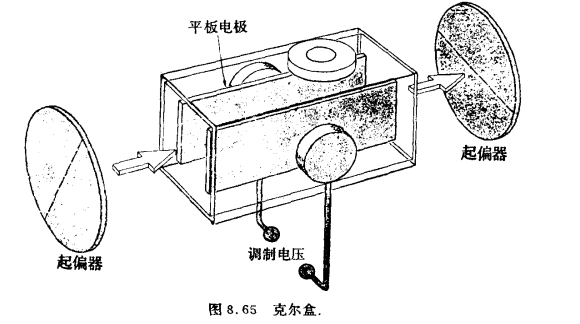
\includegraphics[width=12cm]{KeerBox.png}
	\end{figure}

	对于克尔盒,如果电极板的有效长度为$l$厘米,分开的距离为$d$,那么推迟量为:
	\begin{equation}
	\Delta \varphi=2 \pi K l V^{2} / d^{2}
	\end{equation}
	
	\noindent 式中$V$为外加电压。
	
	还有一个非常重要电光效应,称作泡克耳斯效应,这是一种线性的电光效应。只有不具备中心对称的晶体才有这个效应,所谓不具备中心对称,就是晶体中没有这样的一个中心点,每个原子都可以经过这个中心点反射到一个相同的原子上去。
	\begin{figure}[h]
		\centering
		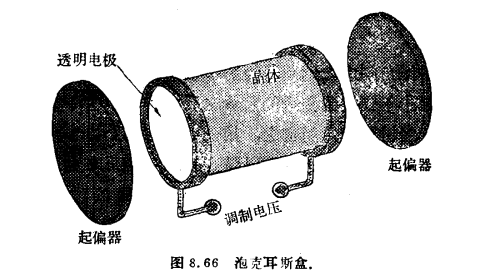
\includegraphics[width=12cm]{PKEBox.png}
	\end{figure}

	晶体本身在不加电场时通常是单轴晶体,并且其光轴沿光束的传播方向。这种装置的推迟量为:
	\begin{equation}
	\Delta \varphi=2 \pi n_{o}^{3} r_{63} V / \lambda_{0}
	\end{equation}
	
	\noindent 其中$r_{63}$是电光常数,单位为米/伏,$n_{0}$是\textbf{寻常}折射率,$V$是以伏特为单位的电位差,$\lambda_{0}$是以米为单位的真空波长。
	
	\section{偏振的数学描述}
	\subsection{斯托克斯参量}
	
	\backdoc
	斯托克斯参量共有四个量,每个量都和一个滤光片相关。假设每个滤光片都在自然光照明下透过一半的光。
	
	现在假定第一个滤光片是简单的各向同性的,仅仅是阻挡一半的光通过;第二个和第三个是线起偏器,其透光轴分别为水平轴和$+45^{\circ}$。最后一个滤光片是圆起偏器,对$\mathscr{L}$态不透明。单独对通过每个滤光片测量透过的辐照度,分别为$I_{0}$,$I_{1}$,$I_{2}$,$I_{3}$,斯托克斯参量的操作定义是:
	\begin{equation}
	\begin{aligned}
	\mathscr{S}_{0}&=2 I_{0}\\
	\mathscr{S}_{1}&=2 I_{1}-2 I_{0}\\
	\mathscr{S}_{2}&=2 I_{2}-2 I_{0}\\
	\mathscr{S}_{3}&=2 I_{3}-2 I_{0}\\
	\end{aligned}
	\end{equation}
	
	可以证明(已经略去了常数):
	\begin{equation}
	\begin{aligned}
	\mathscr{S}_{0}&=\left\langle E_{0 x}^{2}\right\rangle+\left\langle E_{0 y}^{2}\right\rangle\\
	\mathscr{S}_{1}&=\left\langle E_{0 x}^{2}\right\rangle-\left\langle E_{0 y}^{2}\right\rangle\\
	\mathscr{S}_{2}&=\left\langle 2 E_{0 x} E_{0 y} \cos \varepsilon\right\rangle\\
	\mathscr{S}_{3}&=\left\langle 2 E_{0 x} E_{0 y} \sin \varepsilon\right\rangle\\
	\end{aligned}
	\end{equation}
	
	如果光束是非偏振光,$\left\langle E_{0 x}^{2}\right\rangle=\left\langle E_{0 y}^{2}\right\rangle$;由于振幅的平方总归是正的,这两个量哪一个的平均值都不会为零,此时:
	$$
	\mathscr{V}_{0}=\left\langle E_{0 x}^{2}\right\rangle+\left\langle E_{0 y}^{2}\right\rangle, while   \mathscr{S}_{1}=\mathscr{S}_{2}=\mathscr{S}_{3}=0
	$$
	
	对于完全偏振光,可以得到:
	\begin{equation}
	\mathscr{S}_{0}^{2}=\mathscr{S}_{1}^{2}+\mathscr{S}_{2}^{2}+\mathscr{S}_{3}^{2}
	\end{equation}
	
	对于部分偏振光,可以证明偏振度为:
	\begin{equation}
	\boldsymbol{V}=\left(\mathscr{P}_{1}^{2}+\mathscr{S}_{2}^{2}+\mathscr{S}_{3}^{3}\right)^{1 / 2} / \mathscr{S}_{0}
	\end{equation}
	
	对于不相干的波,描述合成波的参量即是元素加法。
	
	\subsection{琼斯矢量}
	
	\backdoc
	琼斯矢量可以作为斯托克斯参量的补充,它只能适用于偏振波。琼斯矢量其实就是电场矢量本身,列矢量形式的琼斯矢量为:
	\begin{equation}
	\mathbf{E}=\left[ \begin{array}{c}{\boldsymbol{E}_{x}(t)} \\ {\boldsymbol{E}_{y}(t)}\end{array}\right]\label{4.23}
	\end{equation}
	
	\noindent 其中$\boldsymbol{E}_{x}(t)$和$\boldsymbol{E}_{y}(t)$是$\boldsymbol{E}$的瞬时标量分量。知道它就知道了偏振态的一切性质,并且如果保留了位相的信息,就可以处理相干波。故可以把 \ref{4.23} 重写为:
	\begin{equation}
	\mathbf{E}=\left[ \begin{array}{c}{\boldsymbol{E}_{0 x} e^{i \varphi_{x}}} \\ {\boldsymbol{E}_{0 y} e^{i \varphi_{y}}}\end{array}\right]
	\end{equation}
	
	对此提出公因式和进行归一化可以得到最简单的琼斯矢量形式。
	
	\subsection{琼斯矩阵和密勒矩阵}
	
	\backdoc
	琼斯矩阵是对琼斯向量进行变换的矩阵,而密勒矩阵是针对斯托克斯向量进行变换的矩阵。两者的变换都是线性变换,同时都遵循左乘规则。
	
	\begin{center}
	\begin{tabular}{c|c|c}
		\toprule
		线性光学元件 & 琼斯矩阵 & 密勒矩阵\\
		
		\midrule
		水平线起偏器 &
		$\left[ \begin{array}{ll}{1} & {0} \\ {0} & {0}\end{array}\right]$
		&
		$\frac{1}{2} \left[ \begin{array}{llll}{1} & {1} & {0} & {0} \\ {1} & {1} & {0} & {0} \\ {0} & {0} & {0} & {0} \\ {0} & {0} & {0} & {0}\end{array}\right]$\\
		
		\midrule
		铅直线起偏器&
		$\left[ \begin{array}{ll}{0} & {0} \\ {0} & {1}\end{array}\right]$
		&
		$\frac{1}{2} \left[ \begin{array}{rrrr}{1} & {-1} & {0} & {0} \\ {-1} & {1} & {0} & {0} \\ {0} & {0} & {0} & {0} \\ {0} & {0} & {0} & {0}\end{array}\right]$\\
		
		\midrule
		$+45^{\circ}$ 线起偏器&
		$\frac{1}{2} \left[ \begin{array}{ll}{1} & {1} \\ {1} & {1}\end{array}\right]$
		&
		$\frac{1}{2} \left[ \begin{array}{llll}{1} & {0} & {1} & {0} \\ {0} & {0} & {0} & {0} \\ {1} & {0} & {1} & {0} \\ {0} & {0} & {0} & {0}\end{array}\right]$\\
		
		\midrule
		$-45^{\circ}$ 线起偏器&
		$\frac{1}{2} \left[ \begin{array}{rr}{1} & {-1} \\ {-1} & {1}\end{array}\right]$
		&
		$\frac{1}{2} \left[ \begin{array}{rrrr}{1} & {0} & {-1} & {0} \\ {0} & {0} & {0} & {0} \\ {-1} & {0} & {1} & {0} \\ {0} & {0} & {0} & {0}\end{array}\right]$\\
		
		\midrule
		四分之一波片,快轴为铅直&
		$e^{i \pi / 4} \left[ \begin{array}{ll}{1} & {0} \\ {0} & {-i}\end{array}\right]$
		&
		$\left[ \begin{array}{llll}{1} & {0} & {0} & {0} \\ {0} & {1} & {0} & {0} \\ {0} & {0} & {0} & {-1} \\ {0} & {0} & {1} & {0}\end{array}\right]$\\
		
		\midrule
		四分之一波片,快轴为水平&
		$e^{i \pi / 4} \left[ \begin{array}{ll}{1} & {0} \\ {0} & {i}\end{array}\right]$
		&
		$\left[ \begin{array}{rrrr}{1} & {0} & {0} & {0} \\ {0} & {1} & {0} & {0} \\ {0} & {0} & {0} & {1} \\ {0} & {0} & {-1} & {0}\end{array}\right]$\\
		
		\midrule
		均匀的圆起偏器,右旋&
		$\frac{1}{2} \left[ \begin{array}{rr}{1} & {i} \\ {-i} & {1}\end{array}\right]$
		&
		$\frac{1}{2} \left[ \begin{array}{llll}{1} & {0} & {0} & {1} \\ {0} & {0} & {0} & {0} \\ {0} & {0} & {0} & {0} \\ {1} & {0} & {0} & {1}\end{array}\right]$\\
		
		\midrule
		均匀的圆起偏器,左旋&
		$\frac{1}{2} \left[ \begin{array}{rr}{1} & {-i} \\ {i} & {1}\end{array}\right]$
		&
		$\frac{1}{2} \left[ \begin{array}{rrrr}{1} & {0} & {0} & {-1} \\ {0} & {0} & {0} & {0} \\ {0} & {0} & {0} & {0} \\ {-1} & {0} & {0} & {1}\end{array}\right]$\\
		
		\bottomrule
	\end{tabular}
	\end{center}
	
	至此,偏振部分的知识梳理可以告一段落了!
\end{document}




